\documentclass[green,xcolor=table,svgnames,hyperref={pdfpagelabels=false},slidestop,usepdftitle=false]{beamer}
\hypersetup{pdfpagemode=FullScreen}
\mode<presentation> {
\usetheme{Warsaw}
\usecolortheme[rgb={ 0.0164,0.6223,0.0164}]{structure}
  \setbeamercovered{transparent}
}
\usepackage{pifont}
\usepackage{amsfonts}
\usepackage{amsmath}
\usepackage{amssymb}
\usepackage[slovak]{babel}
\usepackage{xunicode}
\usepackage{xltxtra}
\usepackage{palatino}
\usepackage{graphicx}

\newenvironment{snimka}{\begin{frame}}{\end{frame}}

\title{Elektronický kompas}
\author[Bc. Michal Srnec]{Bc. Michal Srnec\\Vedúci : doc.Ing.Juraj Miček,PhD}
\institute{Žilinská Univerzita v Žiline\\ Fakulta riadenia a informatiky}
\begin{document}

\begin{frame}
  \titlepage
\end{frame}
\begin{frame}
  \frametitle{Obsah}
  \tableofcontents
\end{frame}

\beamertemplateshadingbackground{white}{white}
\section{Cieľ práce}
\begin{snimka}
 \frametitle{Elektronický kompas - Cieľ}
   \begin{columns}[c]
    \begin{column}{0.4\textwidth}
    \begin{block}{Cieľ}
    \begin{itemize}
         \item Navrhnúť zariadenie, ktoré bude určovať smer azimutu
     \end{itemize}
  \end{block}
   \end{column}
  \end{columns}
      \begin{center}
       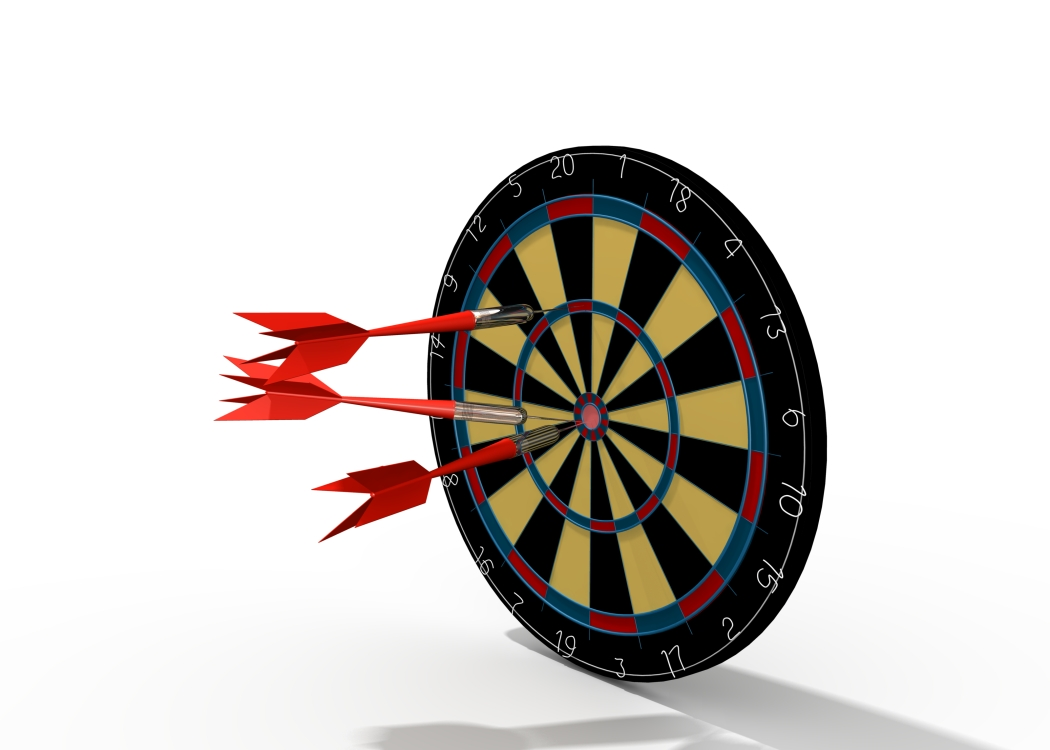
\includegraphics[width=0.85\textwidth]{obr/target1.jpg}
     \end{center}
\end{snimka}
\beamertemplateshadingbackground{white}{white}
\section{Použite}
\begin{snimka}
 \frametitle{Elektronický kompas - Použitie}
   \begin{columns}[c]
    \begin{column}{0.6\textwidth}
     \begin{center}
        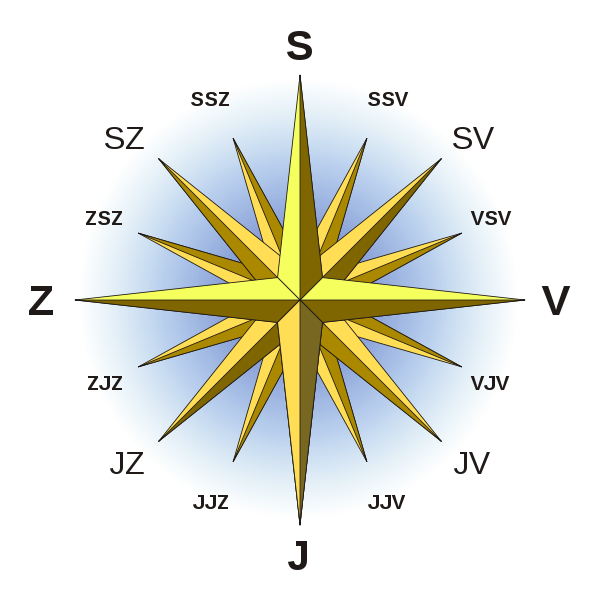
\includegraphics[width=0.8\textwidth]{obr/kompas.png}
      \end{center}
    \end{column}
    \begin{column}{0.4\textwidth}
    \begin{block}{Použitie}
    \begin{enumerate}
         \item Robotika - univerálny modul
         \item Meranie, určovanie azimutu
         \item Nie je možné nasadiť GPS
	\end{enumerate}
  \end{block}
        \end{column}
  \end{columns}
\end{snimka}
\beamertemplateshadingbackground{white}{white}
\section{Požiadavky}
\begin{snimka}
 \frametitle{Elektronický kompas - Požiadavky}
   \begin{columns}[c]
    \begin{column}{0.4\textwidth}
    \begin{block}{Požiadavky}
    \begin{itemize}
         \item Minimalizovať spotrebu
         \item Maximalizovať presnosť
     \end{itemize}
  \end{block}
   \end{column}
    \begin{column}{0.6\textwidth}
     \begin{center}
        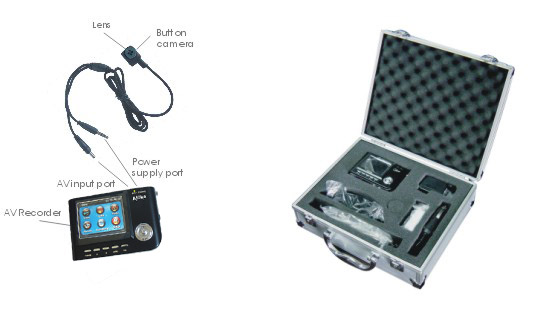
\includegraphics[width=0.9\textwidth]{obr/poziadavky.jpg}
      \end{center}
    \end{column}
  \end{columns}
\end{snimka}
\beamertemplateshadingbackground{white}{white}
\section{Stručný opis}
\begin{snimka}
 \frametitle{Elektronický kompas - Stručný opis}
   \begin{columns}[c]
   \only<1>
   {
    \begin{column}{0.6\textwidth}
     \begin{center}
        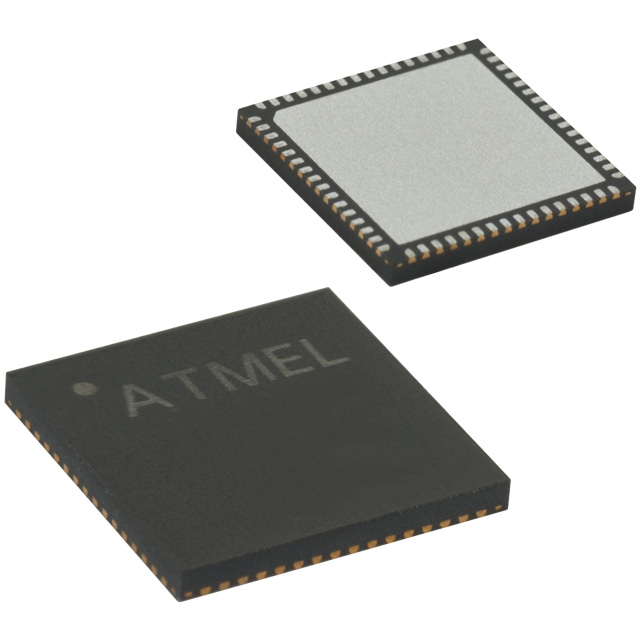
\includegraphics[width=0.8\textwidth]{obr/am7.jpg}
      \end{center}
    \end{column}
    }
   \only<2>
   {
    \begin{column}{0.6\textwidth}
     \begin{center}
        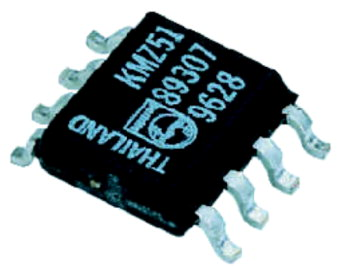
\includegraphics[width=0.8\textwidth]{obr/kmz.jpg}
      \end{center}
    \end{column}
    }

   \only<3>
   {
    \begin{column}{0.6\textwidth}
     \begin{center}
        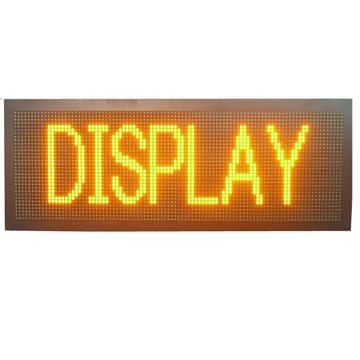
\includegraphics[width=0.8\textwidth]{obr/zobr.jpg}
      \end{center}
    \end{column}
    }

   \only<4>
   {
    \begin{column}{0.6\textwidth}
     \begin{center}
        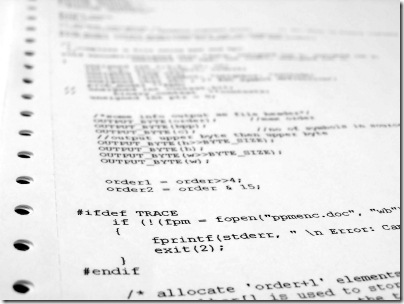
\includegraphics[width=0.8\textwidth]{obr/source.jpg}
      \end{center}
    \end{column}
    }

    \begin{column}{0.4\textwidth}
    \begin{block}{Stručný opis}
    \begin{enumerate}
         \item <+-| alert@+> Výber vhodného MCU.
         \item <+-| alert@+> Senzor, magnetický kompas
         \item <+-| alert@+> Zobrazovanie a vyhodnotovanie výsledkov
         \item <+-| alert@+> Kalibrácia pomocou sw
    \end{enumerate}
  \end{block}
        \end{column}
  \end{columns}
\end{snimka}
\beamertemplateshadingbackground{white}{white}
\section{Bližšie ku senzoru}
\begin{snimka}
 \frametitle{Elektronický kompas - Magnetoresistívny senzor}
   \begin{columns}[c]
    \begin{column}{0.4\textwidth}
    \begin{block}{Magnetoresistívny senzor}
    \begin{itemize}
         \item Princip magnetoresistivneho senzoru
         \item Presnosť, citlivosť
     \end{itemize}
  \end{block}
   \end{column}
    \begin{column}{0.6\textwidth}
     \begin{center}
        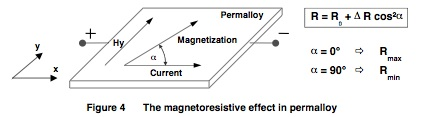
\includegraphics[width=0.7\textwidth]{obr/princip.jpg}
      \end{center}
    \end{column}
  \end{columns}
\end{snimka}
\beamertemplateshadingbackground{white}{white}
\section{Možnosti rozšírenia}
\begin{snimka}
 \frametitle{Elektronický kompas - Možnosti rozšírenia}
   \begin{columns}[c]
    \begin{column}{0.6\textwidth}
     \begin{center}
        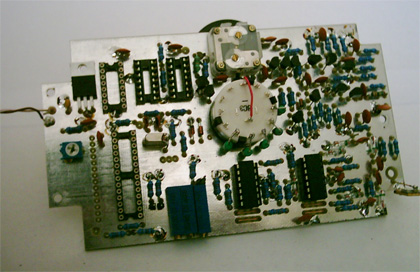
\includegraphics[width=0.8\textwidth]{obr/rozsirenie.jpg}
      \end{center}
    \end{column}
    \begin{column}{0.4\textwidth}
    \begin{block}{Možnosti rozšírenia}
    \begin{itemize}
         \item Gyrosenzor
         \item Meranie iných analógových veličín
	\end{itemize}
  \end{block}
        \end{column}
  \end{columns}
\end{snimka}
\chapter*{Záver}

Cieľom práce bolo navrhnúť riešenie pre vizualizáciu SCADA komponentov vo webovom prehľadači. Mojou úlohou bolo i to, vytvoriť univerzálnejší postup pre animáciu komponentov.  Doterajšie riešenie bolo nepraktické, nebolo to modulárne a vyžadovalo to  zásah do riadiacej časti animácie. Navrhnuté riešenie odstraňuje použitím HTML5 štandardou - SVG, JavaScript. 

Cez Inkscape sa nakreslí komponent, a cez JavaScript pomocou knižnice Snap.svg.js sa manipuluje. Podarilo sa mi aj to, aby bol výsledný prvok responzívny aj na iných platformách ako napríklad tablety. SVG podporujú všetky moderné webové prehliadače.

Moje riešenie používa knižnicu a softvér, ktorý je open-source. Všetky zdrojové kódy práce sú v Git repository na GitHube.
\end{document}